\documentclass[a4paper,11pt]{book}
%\documentclass[a4paper,twoside,11pt,titlepage]{book}
\usepackage{listings}
\usepackage[utf8]{inputenc}
\usepackage[spanish]{babel}

% \usepackage[style=list, number=none]{glossary} %
%\usepackage{titlesec}
%\usepackage{pailatino}

\decimalpoint
\usepackage{dcolumn}
\newcolumntype{.}{D{.}{\esperiod}{-1}}
\makeatletter
\addto\shorthandsspanish{\let\esperiod\es@period@code}
\makeatother


%\usepackage[chapter]{algorithm}
\RequirePackage{verbatim}
%\RequirePackage[Glenn]{fncychap}
\usepackage{fancyhdr}
\usepackage{graphicx}
\usepackage{afterpage}

\usepackage{longtable}

\usepackage[pdfborder={000}]{hyperref} %referencia

% ********************************************************************
% Re-usable information
% ********************************************************************
\newcommand{\myTitle}{Algoritmos meméticos para reducir datos de entrenamiento en modelos de aprendizaje profundo
convolucionales\xspace}
\newcommand{\myDegree}{Grado en Ingeniería Informática\xspace}
\newcommand{\myName}{José Ruiz López (alumno)\xspace}
\newcommand{\myProf}{Daniel Molina Cabrera (tutor)\xspace}
%\newcommand{\mySupervisor}{Put name here\xspace}
\newcommand{\myFaculty}{Escuela Técnica Superior de Ingenierías Informática y de
Telecomunicación\xspace}
\newcommand{\myFacultyShort}{E.T.S. de Ingenierías Informática y de
Telecomunicación\xspace}
\newcommand{\myDepartment}{Departamento de Ciencias de la Computación e Inteligencia Artificial\xspace}
\newcommand{\myUni}{\protect{Universidad de Granada}\xspace}
\newcommand{\myLocation}{Granada\xspace}
\newcommand{\myTime}{\today\xspace}
\newcommand{\myVersion}{Version 0.1\xspace}


\hypersetup{
pdfauthor = {\myName (email (en) ugr (punto) es)},
pdftitle ={\myTitle},
pdfsubject = {},
pdfkeywords = {palabra_clave1, palabra_clave2, palabra_clave3, ...},
pdfcreator = {LaTeX con el paquete ....},
pdfproducer = {pdflatex}
}

%\hyphenation{}


%\usepackage{doxygen/doxygen}
%\usepackage{pdfpages}
\usepackage{url}
\usepackage{colortbl,longtable}
\usepackage[stable]{footmisc}
%\usepackage{index}

%\makeindex
%\usepackage[style=long, cols=2,border=plain,toc=true,number=none]{glossary}
% \makeglossary

% Definición de comandos que me son tiles:
%\renewcommand{\indexname}{Índice alfabético}
%\renewcommand{\glossaryname}{Glosario}

\pagestyle{fancy}
\fancyhf{}
\fancyhead[LO]{\leftmark}
\fancyhead[RE]{\rightmark}
\fancyhead[RO,LE]{\textbf{\thepage}}
\renewcommand{\chaptermark}[1]{\markboth{\textbf{#1}}{}}
\renewcommand{\sectionmark}[1]{\markright{\textbf{\thesection. #1}}}

\setlength{\headheight}{1.5\headheight}

\newcommand{\HRule}{\rule{\linewidth}{0.5mm}}
%Definimos los tipos teorema, ejemplo y definición podremos usar estos tipos
%simplemente poniendo \begin{teorema} \end{teorema} ...
\newtheorem{teorema}{Teorema}[chapter]
\newtheorem{ejemplo}{Ejemplo}[chapter]
\newtheorem{definicion}{Definición}[chapter]

\definecolor{gray97}{gray}{.97}
\definecolor{gray75}{gray}{.75}
\definecolor{gray45}{gray}{.45}
\definecolor{gray30}{gray}{.94}

\lstset{ frame=Ltb,
     framerule=0.5pt,
     aboveskip=0.5cm,
     framextopmargin=3pt,
     framexbottommargin=3pt,
     framexleftmargin=0.1cm,
     framesep=0pt,
     rulesep=.4pt,
     backgroundcolor=\color{gray97},
     rulesepcolor=\color{black},
     %
     stringstyle=\ttfamily,
     showstringspaces = false,
     basicstyle=\scriptsize\ttfamily,
     commentstyle=\color{gray45},
     keywordstyle=\bfseries,
     %
     numbers=left,
     numbersep=6pt,
     numberstyle=\tiny,
     numberfirstline = false,
     breaklines=true,
   }
 
% minimizar fragmentado de listados
\lstnewenvironment{listing}[1][]
   {\lstset{#1}\pagebreak[0]}{\pagebreak[0]}

\lstdefinestyle{CodigoC}
   {
	basicstyle=\scriptsize,
	frame=single,
	language=C,
	numbers=left
   }
\lstdefinestyle{CodigoC++}
   {
	basicstyle=\small,
	frame=single,
	backgroundcolor=\color{gray30},
	language=C++,
	numbers=left
   }

 
\lstdefinestyle{Consola}
   {basicstyle=\scriptsize\bf\ttfamily,
    backgroundcolor=\color{gray30},
    frame=single,
    numbers=none
   }


\newcommand{\bigrule}{\titlerule[0.5mm]}


%Para conseguir que en las páginas en blanco no ponga cabecerass
\makeatletter
\def\clearpage{%
  \ifvmode
    \ifnum \@dbltopnum =\m@ne
      \ifdim \pagetotal <\topskip
        \hbox{}
      \fi
    \fi
  \fi
  \newpage
  \thispagestyle{empty}
  \write\m@ne{}
  \vbox{}
  \penalty -\@Mi
}
\makeatother

\usepackage{pdfpages}
\begin{document}
% !TeX root = ../proyecto.tex

\begin{titlepage}


    \newlength{\centeroffset}
    \setlength{\centeroffset}{-0.5\oddsidemargin}
    \addtolength{\centeroffset}{0.5\evensidemargin}
    \thispagestyle{empty}

    \noindent\hspace*{\centeroffset}\begin{minipage}{\textwidth}

        \centering
        
\includegraphics[width=0.9\textwidth]{imagenes/logo_ugr.jpg}\\[1.4cm]

        \textsc{ \Large TRABAJO FIN DE GRADO\\[0.2cm]}
        \textsc{ INGENIERÍA INFORMATICA }\\[1cm]
        % Upper part of the page
        % 
        % Title
        {\Huge\bfseries Algoritmos meméticos para reducir datos de entrenamiento en modelos de aprendizaje profundo convolucionales\\
        }
        \vspace{0.2cm}
        \noindent\rule[-1ex]{\textwidth}{3pt}\\[3.5ex]
        %{\large\bfseries Subtitulo del Proyecto}
        %\end{minipage}

        \vspace{0.4cm}
        %\noindent\hspace*{\centeroffset}\begin{minipage}{\textwidth}
        %\centering

        \textbf{Autor}\\ {José Ruiz López (alumno)}\\[2.5ex]
        \textbf{Directores}\\
        {Daniel Molina Cabrera (tutor)}\\
        \vspace{0.6cm}
        
\includegraphics[width=0.3\textwidth]{imagenes/etsiit_logo.png}\\[0.1cm]
        \textsc{Escuela Técnica Superior de Ingenierías Informática y de Telecomunicación}\\
        \textsc{---}\\
        Granada, Noviembre de 2024
    \end{minipage}
    %\addtolength{\textwidth}{\centeroffset}
    %\vspace{\stretch{2}}
\end{titlepage}



% !TeX root = ../proyecto.tex

\chapter*{}
%\thispagestyle{empty}
%\cleardoublepage

%\thispagestyle{empty}


\cleardoublepage
\thispagestyle{empty}

\begin{center}
       {\large\bfseries Algoritmos meméticos para reducir datos de entrenamiento en modelos de aprendizaje profundo
              convolucionales}\\
\end{center}
\begin{center}
       José Ruiz López (alumno)\\
\end{center}

%\vspace{0.7cm}
\noindent{\textbf{Palabras clave}: Algoritmos meméticos, Imágenes, Modelos de Aprendizaje profundo convolucionales}\\

\vspace{0.7cm}
\noindent{\textbf{Resumen}}\\

Los \textbf{modelos de Aprendizaje Profundo} (Deep Learning) han supuesto un verdadero hito en la
\textbf{Inteligencia Artificial}, ya que son capaces de procesar grandes volúmenes de datos, además de reconocer
patrones sumamente complejos.
Dentro de estos, los \textbf{modelos convolucionales} se han destacado como particularmente efectivos a la hora de
identificar objetos y características en imágenes, una capacidad esencial para muchas aplicaciones modernas.
Sin embargo, a diferencia de los seres humanos, estos modelos requieren una gran cantidad de datos de
entrenamiento para cada categoría que deben aprender.
Esto implica un proceso de entrenamiento más largo y, muchas veces, la recolección de los datos necesarios puede ser
problemática, según el tipo de información que se necesite.

Además de la dificultad en la obtención de datos,  las nuevas normativas europeas en torno a la inteligencia artificial
establecen la necesidad de auditar no solo los modelos, sino también los datos
utilizados para entrenarlos, especialmente cuando se trata de aplicaciones de IA que manejan datos sensibles.
Estas auditorías, por su propia naturaleza, se volverán más complejas conforme aumente el tamaño del conjunto de
entrenamiento.
Por lo tanto, se vuelve completamente necesario desarrollar estrategias que permitan
\textbf{reducir el tamaño de los conjuntos de datos de entrenamiento} intentado comprometer la calidad del modelo lo mínimo posible.

En este trabajo, proponemos el uso de \textbf{algoritmos meméticos} para establecer un proceso de reducción del conjunto de
\textbf{entrenamiento}, lo que se conoce como \textbf{selección de instancias}.
La idea es seleccionar un conjunto reducido de imágenes representativas que, junto con las técnicas de aumento de
datos, sean suficientes para entrenar modelos convolucionales de manera óptima.
De este modo, se podría reducir significativamente el tamaño del conjunto de entrenamiento, manteniendo la calidad
del aprendizaje y, a su vez, facilitando tanto el proceso de auditoría como la eficiencia computacional del sistema.


\cleardoublepage


\thispagestyle{empty}


\begin{center}
       {\large\bfseries Memetic Algorithms for Reducing Training Data in Convolutional Deep Learning Models}\\
\end{center}
\begin{center}
       José, Ruiz López (student)\\
\end{center}

%\vspace{0.7cm}
\noindent{\textbf{Keywords}: Memetic Algorithms, Images, Convolutional Deep Learning Models}\\

\vspace{0.7cm}
\noindent{\textbf{Abstract}}\\

\textbf{Deep Learning models} have marked a true milestone in the field of \textbf{Artificial Intelligence}, as they are capable of 
processing large volumes of data and recognizing highly complex patterns.
Among these, \textbf{convolutional models} have stood out as particularly effective in identifying objects and
features in images, an essential capability for many modern applications.
However, unlike humans, these models require a large amount of training data for each category they need to learn.
This implies a longer training process, and in many cases, collecting the necessary data can be problematic depending
on the type of information required.

In addition to the difficulty of obtaining data, new European regulations on artificial intelligence establish the need to 
audit not only the models but also the data used to train them, especially in AI applications that handle sensitive data.
These audits, by their very nature, will become increasingly complex as the size of the training set grows.
Therefore, it becomes essential to develop strategies that allow for \textbf{reducing the size of training datasets}, 
while minimizing any compromise in model quality.

In this work, we propose the use of \textbf{memetic algorithms} to implement a \textbf{training data reduction process}, 
also known as \textbf{instance selection}.
The idea is to select a small set of representative images that, along with data augmentation techniques, 
are sufficient to optimally train convolutional models.
In this way, it would be possible to significantly reduce the size of the training set while maintaining learning quality and, 
at the same time, facilitating both the auditing process and the system's computational efficiency.

\chapter*{}
\thispagestyle{empty}

\noindent\rule[-1ex]{\textwidth}{2pt}\\[4.5ex]

Yo, \textbf{José Ruiz López}, alumno de la titulación INGENIERÍA INFORMÁTICA de la \textbf{Escuela Técnica Superior
       de Ingenierías Informática y de Telecomunicación de la Universidad de Granada}, con DNI \textbf{77964364E}, autorizo la
ubicación de la siguiente copia de mi Trabajo Fin de Grado en la biblioteca del centro para que pueda ser
consultada por las personas que lo deseen.

\vspace{6cm}

\noindent Fdo: José Ruiz López

\vspace{2cm}

\begin{flushright}
       Granada a \today.
\end{flushright}


\chapter*{}
\thispagestyle{empty}

\noindent\rule[-1ex]{\textwidth}{2pt}\\[4.5ex]

D. \textbf{Daniel Molina Cabrera (tutor}, Profesor del Departamento Ciencias de la Computación e Inteligencia
Artificial de la Universidad de Granada.

\vspace{0.5cm}

\textbf{Informan:}

\vspace{0.5cm}

Que el presente trabajo, titulado \textit{\textbf{Algoritmos meméticos para reducir datos de entrenamiento en modelos de aprendizaje profundo convolucionales}},
ha sido realizado bajo su supervisión por \textbf{José Ruiz López (alumno)}, y autorizamos la defensa de dicho trabajo  ante el tribunal que corresponda.

\vspace{0.5cm}

Y para que conste, expiden y firman el presente informe en Granada a \today.

\vspace{1cm}

\textbf{Los directores:}

\vspace{5cm}

\noindent \textbf{Daniel Molina Cabrera (tutor)}

\chapter*{Agradecimientos}
\thispagestyle{empty}

\vspace{1cm}


Quiero expresar mi más sincero agradecimiento a todas las personas que han hecho posible la realización de este Trabajo de Fin de Grado.

En primer lugar, me gustaría agradecer al profesor Daniel Molina Cabrera, mi tutor, por su valiosa guía, por su apoyo continuo durante 
todo el proceso y por brindarme acceso a los recursos necesarios para llevar a cabo esta investigación.
Su experiencia y disponibilidad han sido fundamentales para que este proyecto pudiera desarrollarse de forma rigurosa y enriquecedora.

También quiero destacar lo desafiante que ha sido compaginar este trabajo académico con mis responsabilidades laborales.
Ha requerido un esfuerzo constante y una gran capacidad de organización, pero también me ha permitido valorar aún más el proceso y el aprendizaje adquirido.

Agradezco de corazón a mis padres y amigos por su comprensión, paciencia y apoyo emocional durante los momentos más exigentes del camino.
Y, sobre todo, a mi pareja, sin ella no habría sido posible superar el reto que supone realizar un trabajo como este. 
Su apoyo incondicional, su confianza en mí y la calma que me ha transmitido en los momentos más difíciles han sido clave para llegar hasta el final.

Asimismo, extiendo mi gratitud a todas las personas y compañeros que, directa o indirectamente, han contribuido con sus comentarios, sugerencias y tiempo.
Gracias a ellos, este trabajo ha podido alcanzar una mayor profundidad y claridad.

Por último, quiero agradecer a todas aquellas comunidades de código abierto y herramientas libres que han permitido que este proyecto se 
desarrollara sin barreras tecnológicas, facilitando el aprendizaje y la innovación.

\frontmatter
%\tableofcontents
%\listoffigures
%\listoftables
%
\mainmatter
%\setlength{\parskip}{5pt}

% !TeX root = ../proyecto.tex

\chapter{Introducción}\label{ch:introduccion}

%Contexto: Breve introducción al tema y su relevancia.
En la actualidad, vivimos en una era marcada por una constante y acelerada generación de datos.
Este fenómeno ha incrementado la necesidad de desarrollar métodos eficaces para el procesamiento y análisis de grandes
volúmenes de información.
En este contexto, los \textbf{modelos de aprendizaje profundo}, y en particular las
\textbf{redes neuronales convolucionales} (CNN), han demostrado un notable rendimiento en tareas como la
\textbf{clasificación de imágenes}, el \textbf{reconocimiento de patrones} y diversas aplicaciones de alta complejidad.
No obstante, el entrenamiento de estos modelos suele requerir volúmenes elevados de datos, lo que plantea desafíos
significativos tanto en términos de \textbf{tiempo} como de \textbf{costes} asociados a su obtención.



Conforme los sistemas de inteligencia artificial evolucionan hacia estructuras más sofisticadas y precisas, la
disponibilidad de conjuntos de datos amplios y adecuados se vuelve un requisito cada vez más crucial.
Sin embargo, la recopilación, almacenamiento y tratamiento de estos datos suponen obstáculos importantes, especialmente
para aquellas instituciones u organizaciones que cuentan con recursos limitados.
Esta situación pone de relieve la necesidad de investigar estrategias innovadoras que permitan
\textbf{reducir y optimizar los conjuntos de datos} sin comprometer el rendimiento de los modelos entrenados.


En consecuencia, surge la necesidad de \textbf{reducir los conjuntos de datos de entrenamiento}
para mejorar la \textbf{eficiencia} en el desarrollo de modelos de aprendizaje profundo.
Aunque las redes neuronales convolucionales han demostrado un rendimiento notable en diversas tareas, su implementación
conlleva \textbf{altos costes computacionales} y una gran demanda de datos, lo que  supone un obstáculo importante en muchos escenarios,
especialmente aquellos con recursos limitados.
Una estrategia prometedora consiste en entrenar estos modelos utilizando únicamente una fracción de los datos
disponibles, seleccionados de manera óptima.
Esta aproximación permitiría disminuir significativamente el consumo de recursos sin comprometer la precisión del
modelo, lo que supondría un avance importante para la \textbf{inteligencia artificial}, en particular en aplicaciones
donde existen \textbf{restricciones de recursos}.


En este contexto, la selección inteligente de subconjuntos representativos constituye una estrategia eficaz para reducir tanto
los tiempos de entrenamiento como el uso de recursos, sin afectar negativamente el rendimiento.
Es precisamente en este punto donde las \textbf{metaheurísticas} adquieren un papel relevante.
Estas técnicas de optimización están diseñadas para abordar problemas complejos en los que los métodos tradicionales
resultan ineficaces, gracias a sus \textbf{estrategias de búsqueda} y \textbf{exploración del espacio de soluciones}.
Al combinar diversas heurísticas, permiten encontrar soluciones aproximadas en tiempos razonables, lo que las convierte
en una herramienta especialmente útil cuando la obtención de una solución exacta resulta inviable desde el punto de
vista computacional.


Gracias a estas características, las metaheurísticas se posicionan como una alternativa sólida
para mejorar la eficiencia y accesibilidad del aprendizaje profundo, incluso en contextos con recursos limitados.
Esto es especialmente relevante para avanzar hacia una inteligencia artificial más abierta, \textbf{democrática} y aplicable
en una mayor variedad de escenarios.


En este contexto, el presente Trabajo de Fin de Grado tiene como objetivo aplicar técnicas metaheurísticas para realizar una selección
inteligente de ejemplos, con el fin de reducir el tamaño de los conjuntos de entrenamiento sin que ello afecte
significativamente a los resultados obtenidos.
La investigación aspira a contribuir al desarrollo de modelos más \textbf{eficientes}, accesibles y económicamente
sostenibles, fomentando así un futuro en el que la inteligencia artificial sea más \textbf{inclusiva} y
\textbf{sostenible}.


%Objetivos: Especifica qué pretendes lograr con tu TFG.
El objetivo principal de este TFG es investigar la aplicación de \textbf{metaheurísticas} para la
\textbf{reducción de conjuntos de datos de entrenamiento} en modelos de \textbf{aprendizaje profundo convolucionales}.
Este estudio permitirá evaluar el impacto de dichos algoritmos en la \textbf{eficiencia computacional} y en el
\textbf{rendimiento de los modelos}.
Para lograr estos objetivos, se desarrollarán y compararán distintas técnicas de selección de instancias aplicadas
sobre modelos convolucionales, incluyendo enfoques aleatorios, de búsqueda local, genéticos y meméticos.


Para cumplir con este objetivo general, se plantean los siguientes \textbf{objetivos específicos}:

\begin{itemize}
      \item \textbf{Estudiar} la conveniencia del uso de metaheurísticas para la reducción de conjuntos de imágenes
            en modelos de aprendizaje profundo.
      \item \textbf{Desarrollar} y \textbf{mejorar} algoritmos metaheurísticos orientados a la selección de ejemplos representativos,
            con el objetivo de optimizar el entrenamiento de modelos convolucionales sin comprometer su rendimiento.
      \item \textbf{Evaluar} el impacto de la reducción de datos en el rendimiento de los modelos, comparando aspectos clave
            como la precisión, eficacia y el tiempo de entrenamiento, en modelos entrenados con conjuntos de datos completos frente a conjuntos reducidos.
      \item \textbf{Comparar} el rendimiento de metaheurísticas con porcentajes de selección fijos frente a aquellos que
            permiten una selección flexible del número de ejemplos, analizando sus ventajas y limitaciones.
\end{itemize}

A través de este estudio, se busca no solo mejorar el rendimiento y la eficiencia de los modelos convolucionales,
sino también fomentar el desarrollo de soluciones más \textbf{sostenibles y accesibles} en el ámbito de la inteligencia artificial,
mediante la incorporación de estrategias metaheurísticas como \textbf{propuestas innovadoras} para la reducción de datos de entrenamiento.

Este trabajo se enmarca en el Proyecto ``Inteligencia Artificial Ética, Responsable y de Propósito General: Aplicaciones En Escenarios De Riesgo.'' (IAFER) Exp.:TSI-100927-2023-1.


%\input{capitulos/02_EspecificacionRequisitos}

%\input{capitulos/03_Planificacion}
%
%\input{capitulos/04_Analisis}

\input{capitulos/05_Diseño}

%% !TeX root = ../proyecto.tex

\chapter{Implementación}\label{ch:implementacion}
En este capítulo se presenta en detalle la arquitectura técnica del sistema implementado, incluyendo los componentes y
módulos principales, las herramientas específicas empleadas en la construcción del sistema, y los elementos clave para
optimizar el rendimiento de los algoritmos y su evaluación.


\section{Descripción del Sistema}\label{sec:descripcion-del-sistema}
%Descripción del Sistema: Detalla la arquitectura del sistema que estás implementando.
La estructura del proyecto se organizó modularmente para facilitar el acceso, el mantenimiento y la extensibilidad del código fuente.
La organización de carpetas es la siguiente:
\begin{itemize}
      \item \texttt{data} -- Conjunto de datos utilizados en los experimentos.
      \item \texttt{docs} -- Documentación del proyecto en latex.
            \begin{itemize}
                  \item \texttt{bibliografia} -- Archivos relacionados con las referencias bibliográficas.
                  \item \texttt{capitulos} -- Archivos individuales para cada capítulo del documento.
                  \item \texttt{config} -- Archivos de configuraciones de la documentación LaTeX.
                  \item \texttt{imagenes} -- Imágenes utilizadas en la documentación.
                  \item \texttt{out} -- Archivos generados por el compilador de LaTeX.
                  \item \texttt{portada} -- Archivo portada del documento.
                  \item \texttt{prefacio} -- Archivo prefacio del documento.
                  \item \texttt{proyecto.tex} -- Archivo principal de LaTeX que compila el documento.
            \end{itemize}
      \item \texttt{img} -- Imágenes generadas automáticamente durante los experimentos.
      \item \texttt{LICENSE} -- Términos de distribución del proyecto.
      \item \texttt{logs} -- Registros de las ejecuciones, incluyendo tiempos de inicio, fin y resultados intermedios de los algoritmos.
      \item \texttt{README.md} -- Descripción general.
      \item \texttt{requirements.txt} -- Dependencias del proyecto.
      \item \texttt{results} -- Resultados de los experimentos.
            \begin{itemize}
                  \item \texttt{csvs} -- Resultados de las ejecuciones guardados en tablas.
                  \item \texttt{salidas} -- Salidas en bruto de consola.
            \end{itemize}
      \item \texttt{scripts} -- Scripts de ejecución automática, comparación de experimentos y generación de gráficos finales.
      \item \texttt{src} -- Código fuente principal del proyecto.
            \begin{itemize}
                  \item \texttt{algorithms} -- Implementaciones de los algoritmos.
                  \item \texttt{main.py} -- Módulo principal de ejecución individual.
            \end{itemize}
      \item \texttt{tmp} -- Ficheros temporales generados durante la ejecución.
      \item \texttt{utils} -- Módulos de apoyo, como clases auxiliares, generación de gráficos y funciones utilitarias.
\end{itemize}

El código completo del proyecto, incluyendo los scripts, algoritmos, documentación y resultados,
se encuentra disponible en el repositorio público de GitHub: \url{https://github.com/JoseRuizLopez/TFG}.


\section{Herramientas y Lenguajes de Programación}\label{sec:herramientas-y-lenguajes-de-programacion}
%Herramientas y Lenguajes de Programación: Lista las herramientas y tecnologías que usarás.
El desarrollo del proyecto se ha llevado a cabo utilizando \textbf{Python 3.10}~\cite{vanderplasPythonDataScience2016} como
lenguaje principal, debido a su versatilidad y amplia adopción en el campo del \textbf{aprendizaje profundo} y la
\textbf{manipulación de datos}.
Python es conocido por su facilidad de uso, extensibilidad y la gran cantidad de bibliotecas disponibles para el
procesamiento de datos y la implementación de modelos de \textbf{machine learning}.


Las principales bibliotecas empleadas durante el desarrollo son las siguientes:
\begin{itemize}
      \item \textbf{PyTorch 2.3.1}~\cite{ketkarIntroductionPyTorch2021, TorchcudaPyTorch24}: Para la construcción,
            entrenamiento y optimización de modelos de aprendizaje profundo.
            PyTorch fue elegido por su flexibilidad y capacidad para ejecutarse eficientemente en GPU\@.
      \item \textbf{Scikit-learn 1.5.2}~\cite{vanderplasPythonDataScience2016}: Para la evaluación de los modelos se utilizaron
            métricas estándar~\cite{kramerScikitLearn2016}.
            Su API permite una integración fluida con PyTorch y otros módulos.
      \item \textbf{Numpy 2.0.0}~\cite{NumPyV20Manual}: Para operaciones matemáticas y manipulación de matrices,
            siendo una herramienta esencial en el procesamiento de datos.
      \item \textbf{Polars 1.9.0}~\cite{PolarsPythonAPI}: Biblioteca para manejar DataFrames de gran tamaño,
            elegida por su rendimiento superior en comparación con Pandas.
      \item \textbf{Matplotlib 3.9.2}~\cite{Matplotlib393Documentation}: Biblioteca utilizada para la generación y
            visualización de gráficas.
      \item \textbf{Seaborn 0.13.2}~\cite{Seaborn0132Documentation}: Estilización avanzada de gráficos estadísticos.
      \item \textbf{Openpyxl 3.1.5}~\cite{Openpyxl313Documentation}: Generación automática de archivos Excel a partir de resultados experimentales.
\end{itemize}

Cada una de estas herramientas fue seleccionada por su robustez y su idoneidad para cumplir con los requisitos
específicos del proyecto, facilitando tanto la implementación de los algoritmos meméticos como la reducción y el
análisis de los datos utilizados en los modelos de aprendizaje profundo.

\section{Gestión de Dependencias}\label{sec:gestion-de-dependencias}
Para garantizar que el proyecto se ejecute correctamente y todas las bibliotecas necesarias estén disponibles, se ha
utilizado un archivo \texttt{requirements.txt}.
Este archivo contiene una lista de todas las bibliotecas y sus versiones específicas que el proyecto requiere.


Para el \textbf{desarrollo local}, se ha optado por crear un entorno virtual utilizando
\texttt{venv}~\cite{CreationVirtualEnvironments}.
Esta práctica permite aislar las dependencias del proyecto de otros proyectos en la máquina, evitando conflictos entre
versiones de bibliotecas.


Para la \textbf{implementación en el servidor}, se ha utilizado \texttt{conda}~\cite{CondaDocumentation} como gestor
de paquetes y entornos.
Conda facilita la gestión de entornos y la instalación de bibliotecas, especialmente en configuraciones más complejas.



Esto facilita la reproducibilidad del proyecto y minimiza posibles conflictos de versión, lo que es fundamental para
mantener la integridad del código y el rendimiento de las aplicaciones.

\section{Arquitectura de la Implementación}\label{sec:arquitectura-de-la-implementacion}
La arquitectura de la implementación desarrollada para este trabajo está diseñada con un enfoque modular y escalable,
que permite gestionar de forma eficiente las distintas fases del proceso de selección de instancias y evaluación de modelos.
El sistema se compone de varios módulos interrelacionados que se encargan de la generación de subconjuntos,
la ejecución de los algoritmos evolutivos y meméticos, la evaluación de las soluciones mediante modelos preentrenados, y la visualización y almacenamiento de resultados.
Esta estructura facilita la incorporación de nuevos algoritmos o mejoras en los ya existentes, garantizando una mayor flexibilidad y mantenimiento del código.

\subsection{Esquema General de Funcionamiento de los Algoritmos}\label{subsec:esquema-algoritmos}
El funcionamiento general de los algoritmos implementados en este trabajo sigue un flujo estructurado y modular que permite una ejecución ordenada de todas las etapas del proceso.
La Figura~\ref{fig:esquema-flujo-algoritmos} muestra el esquema general de funcionamiento, desde la configuración inicial hasta la evaluación final de resultados.

\begin{figure}[htp]
      \centering
      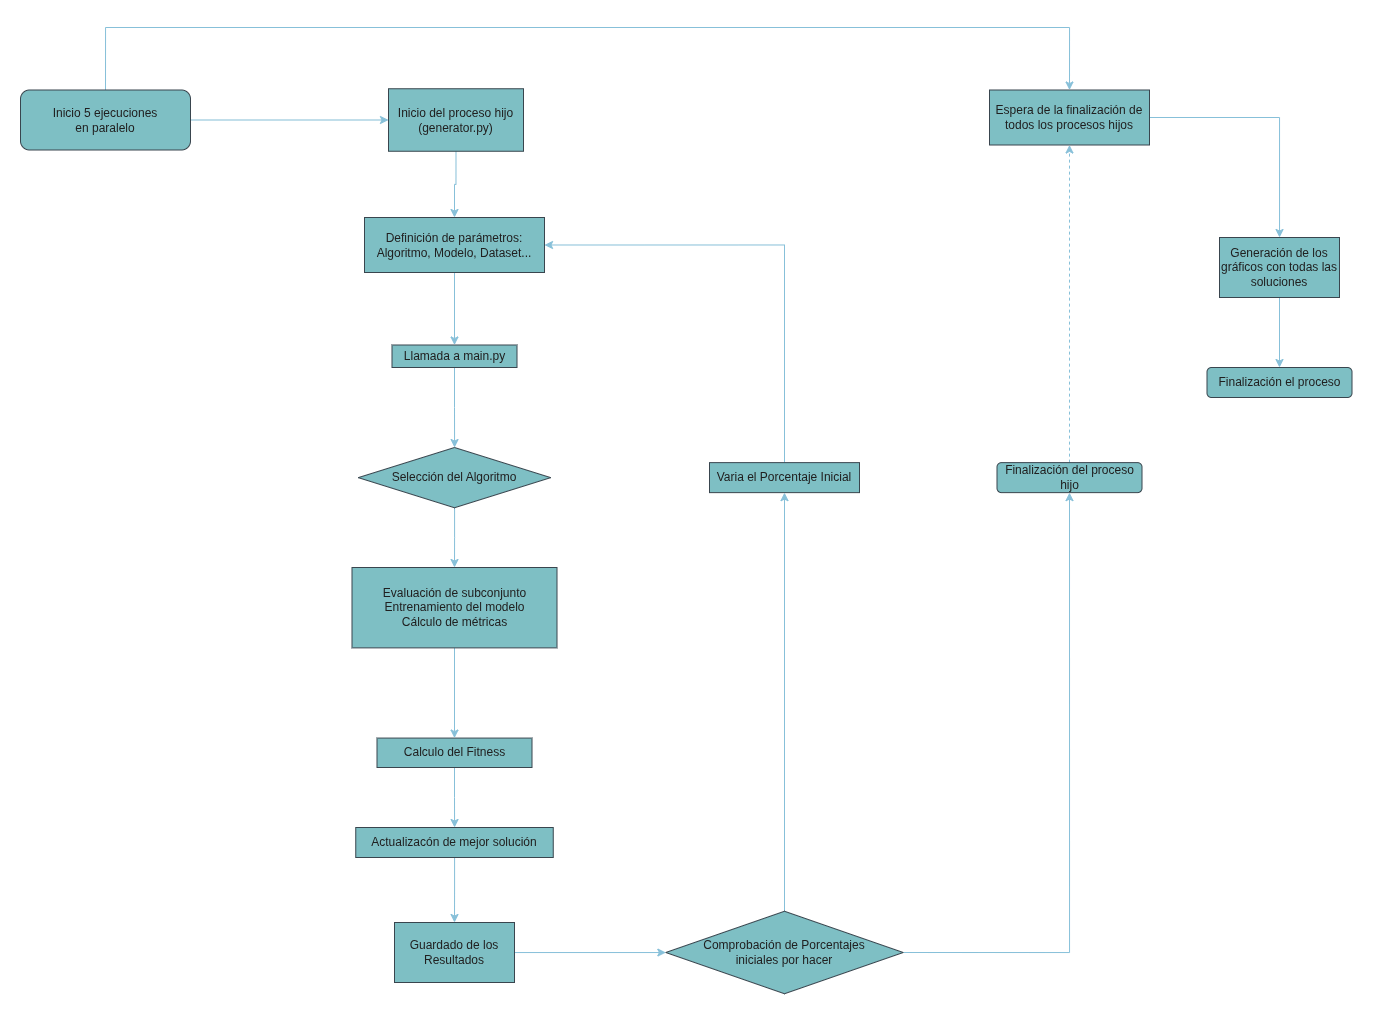
\includegraphics[width=0.95\textwidth]{imagenes/flujo2.drawio}
      \caption{Esquema general del flujo de ejecución de los algoritmos y evaluación de subconjuntos.}
      \label{fig:esquema-flujo-algoritmos}
\end{figure}

El proceso se organiza en los siguientes pasos principales:

\begin{enumerate}
      \item \textbf{Ejecución del script de paralelización:} Se inicia el script que permite ejecutar múltiples experimentos de manera paralela,
            facilitando la obteción de resultados de diferentes semillas.
      \item \textbf{Configuración inicial:} Se define el algoritmo, el modelo y el dataset a utilizar, a través de los parámetros en \texttt{generator.py}.
      \item \textbf{Ejecución del núcleo principal:} El script \texttt{main.py} se encarga de orquestar la ejecución,
            llamando a las funciones específicas según el algoritmo seleccionado.
      \item \textbf{Generación y evaluación de subconjuntos:} Cada algoritmo genera subconjuntos de datos de entrenamiento a partir del conjunto original.
      \item \textbf{Entrenamiento del modelo:} Se realiza el entrenamiento del modelo utilizando los subconjuntos generados,
            aplicando técnicas de \textit{transfer learning} con modelos preentrenados.
      \item \textbf{Almacenamiento de resultados:} Cada evaluación almacena los resultados obtenidos (métricas y composición del subconjunto) y,
            tras finalizar la ejecución, se generan gráficos como boxplots y visualizaciones que permiten analizar el rendimiento de cada enfoque.
\end{enumerate}

\subsection{Configuración de Modelos Preentrenados}\label{subsec:configuracion-modelos-preentrenados}
En este trabajo, se han utilizado modelos convolucionales preentrenados como base para la tarea de clasificación de imágenes.
Concretamente, se han empleado las arquitecturas \textbf{ResNet50} y \textbf{MobileNetV2},
cargadas con pesos preentrenados sobre \texttt{ImageNet} o \texttt{CIFAR10}, según el dataset utilizado en cada experimento.

Para adaptar estos modelos a la tarea específica de clasificación de subconjuntos de datos,
se ha seguido una estrategia de \textit{transfer learning} que permite reducir significativamente el coste computacional del entrenamiento.
Esta estrategia consiste en congelar todas las capas del modelo, excepto la última,
de manera que las representaciones aprendidas en la etapa preentrenada puedan ser reutilizadas como extractores de características generales.

Específicamente, la \textbf{última capa} de cada modelo preentrenado (la capa densa o \textit{fully connected})
ha sido reemplazada por una nueva capa completamente conectada (\texttt{Linear}) adaptada al número de clases del dataset en uso.
Esta capa es la única que se entrena durante la fase de evaluación de cada subconjunto generado por los algoritmos,
permitiendo obtener métricas como \textit{accuracy}, \textit{precision}, \textit{recall} y \textit{F1-score} de forma eficiente.

El uso de pesos preentrenados y la congelación de capas proporcionan varias ventajas:
\begin{itemize}
      \item Reducción del tiempo de entrenamiento en cada evaluación.
      \item Aprovechamiento de representaciones genéricas previamente aprendidas, lo que mejora la generalización.
      \item Adaptabilidad de los modelos a distintos datasets y tareas, modificando únicamente la capa final.
\end{itemize}

Este enfoque se implementa mediante las herramientas de PyTorch,
congelando explícitamente los gradientes de todas las capas del modelo y definiendo la nueva capa final con el número adecuado de salidas para cada problema de clasificación.

\subsection{Módulo de Algoritmos}\label{subsec:modulo-de-algoritmos}
Ubicado en \texttt{src/algorithms/} este módulo contiene las implementaciones principales de los
algoritmos desarrollados en el proyecto.

Este módulo utiliza la arquitectura GPU para maximizar la velocidad de ejecución y está diseñado para ser escalable,
permitiendo la inclusión de nuevos operadores meméticos si es necesario.

\subsection{Núcleo de Ejecución}\label{subsec:nucleo-de-ejecucion}
El módulo \texttt{main.py} centraliza la ejecución de un experimento individual, inicializando configuraciones,
entrenando el modelo y generando gráficos.

Los pasos de la función principal de \texttt{main.py} es:
\begin{enumerate}
      \item \textbf{Establece Configuración Inicial}: Configura una semilla, elige el dataset y prepara un archivo de log.
      \item \textbf{Inicia el Proceso del Algoritmo}: Según el nombre del algoritmo (algoritmo) especificado, se llama a
            la función correspondiente (por ejemplo, genetic\_algorithm, memetic\_algorithm, etc.).
      \item \textbf{Almacena Resultados}: Una vez que el algoritmo termina, registra la duración, los resultados y la
            métrica final en un archivo.
      \item \textbf{Visualiza Resultados}: Si hay datos de fitness, genera una gráfica de la evolución del fitness a lo
            largo del proceso.
      \item \textbf{Genera un Resumen}: Calcula estadísticas adicionales (como porcentaje de clases seleccionadas en
            Paper, Rock y Scissors), y devuelve estos resultados junto con el historial de fitness.
\end{enumerate}

\subsection{Módulo de Utilidades}\label{subsec:modulo-de-utilidades}
La carpeta \texttt{utils/} contiene funciones auxiliares:
\begin{itemize}
      \item \textbf{utils\_plot.py}: Generación de gráficos.
      \item \textbf{classes.py}: Definición de enumeraciones para algoritmos, métricas, datasets y modelos.
      \item \textbf{utils.py}: Funciones de ayuda como el cálculo de métricas o la creación de diccionarios de selección de imágenes.
\end{itemize}

Estos módulos se encargan de generar gráficas comparativas entre distintos porcentajes o algoritmos y en
generar un CSV con los datos finales para ser analizados.

\subsection{Scripts de Ejecución en GPU}\label{subsec:scripts-de-ejecucion-en-gpu}
En scripts, se encuentran los programas necesarios para ejecutar los algoritmos en un servidor GPU, lo que permite
maximizar la eficiencia en el entrenamiento y la evaluación de modelos.
\begin{enumerate}
      \item \textbf{Configuración de GPU}: Los scripts están configurados para identificar y utilizar las GPU disponibles
            en el servidor, reduciendo los tiempos de entrenamiento de modelos.
      \item \textbf{Optimización de Ejecución}: Se implementaron configuraciones de batch size y técnicas de
            procesamiento paralelo en PyTorch, aprovechando la memoria y el poder de procesamiento de las GPU\@.
\end{enumerate}

Estos scripts están diseñados para ser ejecutados en un entorno de servidor, reduciendo los tiempos de prueba en el
entorno local y permitiendo un análisis iterativo más rápido.

\section{Consideraciones de Optimización}\label{sec:consideraciones-de-optimizacion}
Durante el desarrollo, se optimizaron varios aspectos para mejorar el rendimiento del sistema:

\begin{enumerate}
      \item \textbf{Aceleración en GPU}: Todas las operaciones de cálculo intensivo fueron migradas a la GPU mediante
            PyTorch.
      \item \textbf{Uso Eficiente de Memoria}: Con Polars y Numpy, se optimizó el manejo de grandes volúmenes de datos,
            utilizando tipos de datos específicos para reducir el uso de memoria.
      \item \textbf{Automatización de Evaluaciones}: Las pruebas de rendimiento se automatizaron, permitiendo una
            evaluación continua sin intervención manual.
      \item \textbf{Control de reproducibilidad}: Se fijaron semillas aleatorias en todas las librerías involucradas
            (random, numpy, torch, cuda) y se desactivaron los algoritmos no deterministas de cuDNN~\cite{CuBLASDeterministicAlgorithms}.
            Esta medida garantiza que las ejecuciones del sistema produzcan resultados consistentes entre sesiones,
            algo esencial en entornos de evaluación comparativa.
      \item \textbf{Diagnóstico automático de GPU}: Implementación de un script (cuda-diagnostic.py) que comprueba disponibilidad
            de CUDA y dispositivos antes de lanzar experimentos, garantizando un entorno correcto.
\end{enumerate}

Además, se implementó un mecanismo de \textbf{early stopping} basado en la ausencia de mejora del valor de fitness durante
un número determinado de evaluaciones consecutivas.
Aunque no se utiliza una pérdida de validación explícita como en enfoques tradicionales, este enfoque funcionalmente cumple el mismo propósito:
detener el algoritmo cuando se detecta estancamiento, reduciendo así el coste computacional innecesario~\cite{EarlyStoppingDiscussion2024}.


Gracias a estas optimizaciones, el sistema permite explorar un amplio abanico de configuraciones de manera eficiente, manteniendo la robustez y estabilidad de los resultados.

\section{Métricas de Evaluación}\label{sec:metricas-evaluacion}

Para evaluar el rendimiento de los modelos de clasificación utilizados en los experimentos,
se han empleado cuatro métricas estándar en el ámbito del aprendizaje automático: \textbf{accuracy}, \textbf{precisión}, \textbf{recall} y \textbf{F1-score}.
Dado que se trata de un problema multiclase, estas métricas se han calculado utilizando el promedio \textit{macro},
lo que implica computarlas individualmente para cada clase y luego obtener la media aritmética.

A continuación se describen y formalizan cada una de estas métricas:

\begin{itemize}
      \item \textbf{Accuracy} (exactitud): representa la proporción de predicciones correctas sobre el total de ejemplos.
            $$
                  Accuracy = \frac{TP + TN}{TP + TN + FP + FN}
            $$
            En el caso multiclase, se generaliza como:
            $$
                  \mathrm{Accuracy} = \frac{\text{Número de predicciones correctas}}{\text{Total de predicciones}}
            $$

      \item \textbf{Precisión}: mide cuántas de las instancias clasificadas como positivas fueron realmente positivas.
            En el caso multiclase (macro), se calcula como:
            $$
                  \text{Precisión}_{\text{macro}} = \frac{1}{C} \sum_{i=1}^{C} \frac{TP_i}{TP_i + FP_i}
            $$

      \item \textbf{Recall}: indica cuántas de las instancias realmente positivas fueron correctamente identificadas por el modelo:
            $$
                  \mathrm{Recall}_{\text{macro}} = \frac{1}{C} \sum_{i=1}^{C} \frac{TP_i}{TP_i + FN_i}
            $$

      \item \textbf{F1-score}: es la media armónica entre precisión y recall, útil cuando se desea un equilibrio entre ambas:
            $$
                  \mathrm{F1\text{-}score}_{\text{macro}} = \frac{1}{C} \sum_{i=1}^{C} \frac{2 \cdot \text{Precisión}_i \cdot \text{Recall}_i}{\text{Precisión}_i + \text{Recall}_i}
            $$
\end{itemize}

Donde:
\begin{itemize}
      \item $TP_i$: verdaderos positivos de la clase $i$
      \item $FP_i$: falsos positivos de la clase $i$
      \item $FN_i$: falsos negativos de la clase $i$
      \item $C$: número total de clases
\end{itemize}

Para facilitar la comprensión de estos conceptos, en la Figura~\ref{fig:matriz-confusion} se muestra una representación gráfica de una matriz de confusión.
\begin{figure}[H]
      \centering
      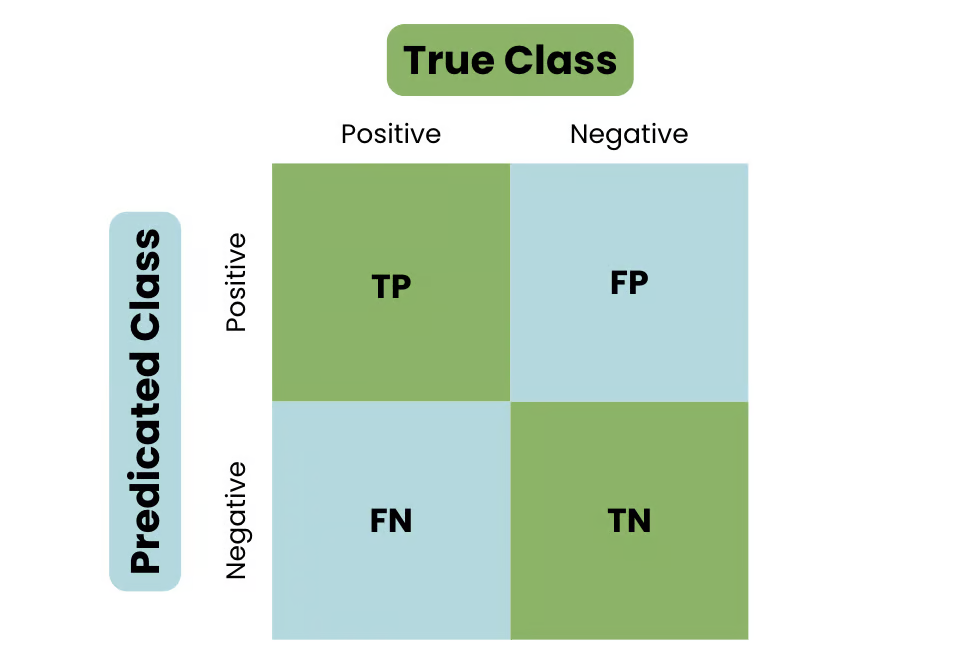
\includegraphics[width=0.5\textwidth]{imagenes/matriz-de-confusion.png}
      \caption{Representación gráfica de una matriz de confusión}
      \label{fig:matriz-confusion}
\end{figure}

Estas métricas fueron implementadas utilizando la librería \texttt{scikit-learn}, que permite su cálculo eficiente a partir de las
predicciones del modelo y las etiquetas reales del conjunto de validación.

%
%\input{capitulos/07_Pruebas}
%
%% !TeX root = ../proyecto.tex

\chapter{Conclusiones}\label{ch:conclusiones}
%
%%\chapter{Conclusiones y Trabajos Futuros}
%
%
%%\nocite{*}
%\bibliography{bibliografia/bibliografia}\addcontentsline{toc}{chapter}{Bibliografía}
%\bibliographystyle{miunsrturl}
%
%\appendix
%\input{apendices/manual_usuario/manual_usuario}
%%\input{apendices/paper/paper}
%\input{glosario/entradas_glosario}
% \addcontentsline{toc}{chapter}{Glosario}
% \printglossary
\chapter*{}
\thispagestyle{empty}

\end{document}
